For purpose of showing some functionality for potential customers of the final solution, it was chosen to construct a vertical prototype of the smartphone application.

The prototype implemented some of the key functionality, still leaving some functionality. The purpose of this is to show a small set of complete functionality. The application was supposed to look like the paper prototype described in \cref{paper_prototype}. Some of the design functionality were not implemented or replaced with a dummy button just to show the potential design.

\begin{figure}[h!]
  \centering
  \subfloat[An example search in the prototype]{
    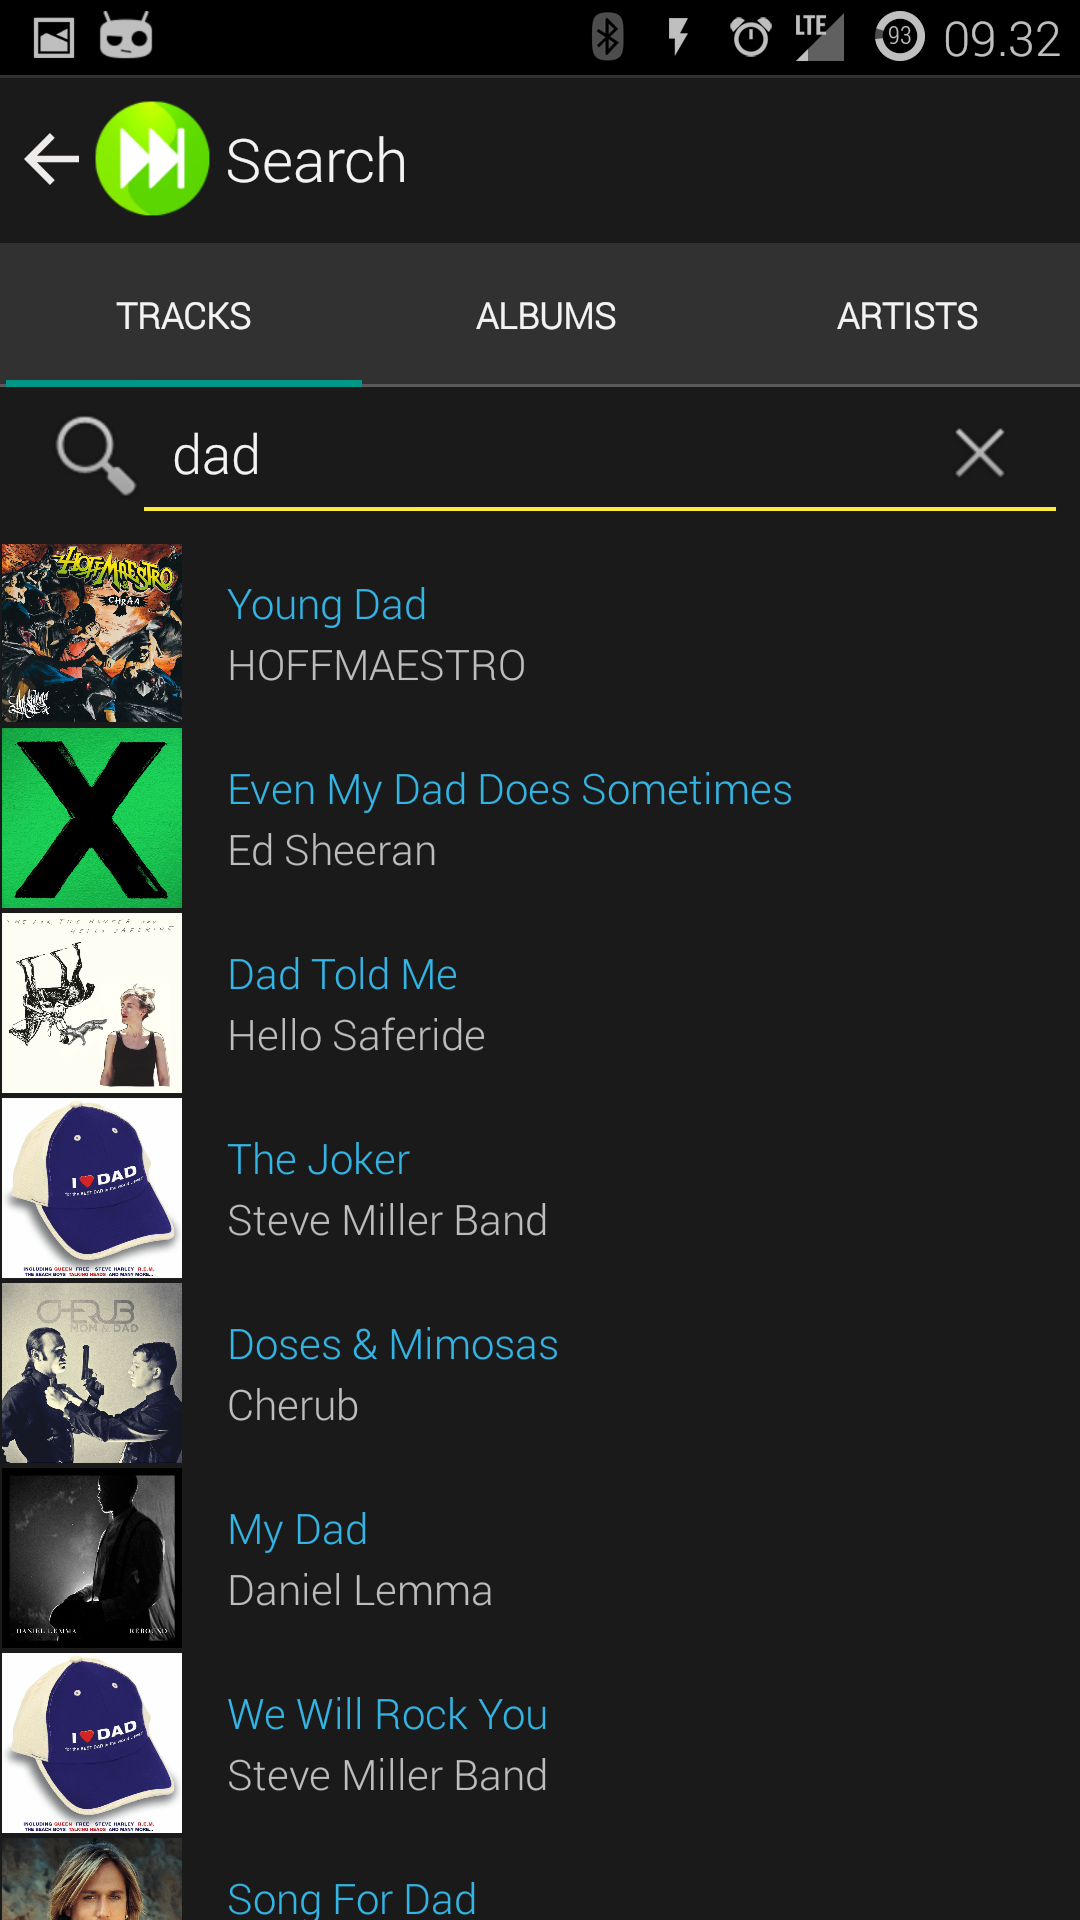
\includegraphics[width=0.5\textwidth]{searchResult}
    \label{fig:searchResult}
  }
  \subfloat[In this early prototype the user still needed to enter the IP manually]{
    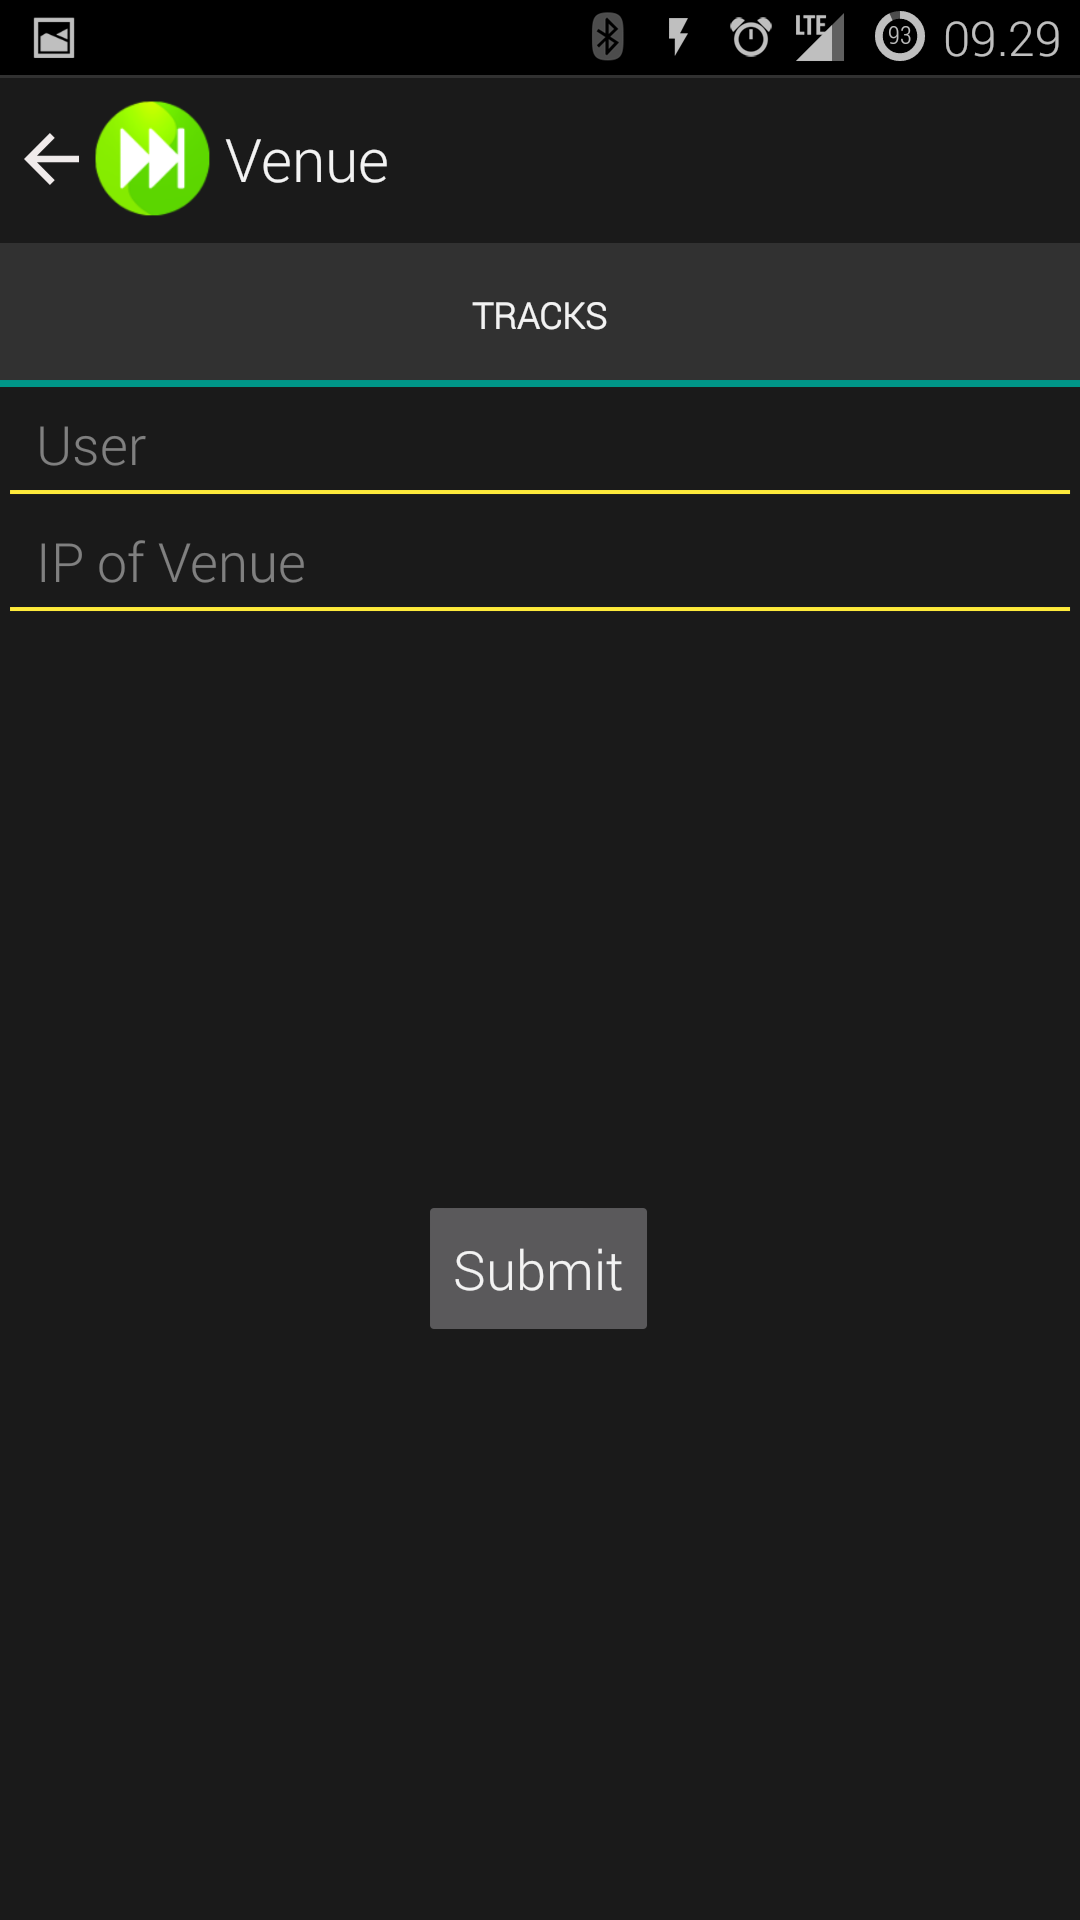
\includegraphics[width=0.5\textwidth]{ipScreen}
    \label{fig:ipScreen}
  }
  \caption{Screenshots from the prototype shown to \enquote{Fabrikken}}
\end{figure}

\subsection{Vertical Prototype}
\label{sub:vertical_prototype}
The prototype was designed for android phones, which is one of the mobile phones that the application is supposed to support. Some of the functionality implemented are listed below. 

\frnote{mere her}